\subsection{Instalación de Java}   
%% Instalacion de Java El primer paso es ejecutar el archivo
Descargado, recuerde que no importa la versión del JDK que haya descargado,
puede ser una versión anterior o posterior (Recomendamos la \textit{versión 8}).

\begin{figure}[H]
	\begin{center}
		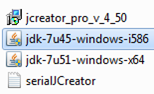
\includegraphics[scale=.4]{images/instalaciones/java/img_java_1}
		\caption{Archivo ejecutable o instalador.}
	\end{center}
\end{figure} 

 Al ejecutar este archivo nos desplegará la siguiente ventana de
bienvenidos al instalador de actualización del JDK.    

\begin{figure}[H]
	\begin{center}
		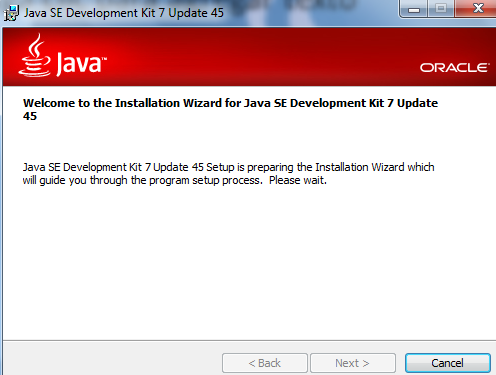
\includegraphics[scale=.4]{images/instalaciones/java/img_java_2}
		\caption{Ventana inicial para comenzar la instalación.}
	\end{center}
\end{figure} 

 A los pocos
segundos nos mostrara la imagen de bienvenida al instalador de JDK, el
procedimiento es verificar si existe en su equipo de cómputo una versión
anterior a instalar, si existe dicha versión de JDK solo actualizara su JDK de
lo contrario será una instalación desde cero, en la que deberemos dar clic en
aceptar para que inicie el proceso de instalación.

\begin{figure}[H]
	\begin{center}
		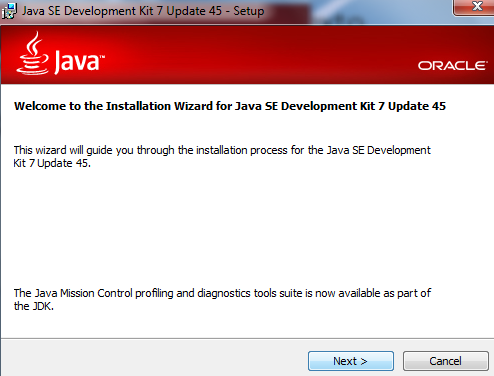
\includegraphics[scale=.4]{images/instalaciones/java/img_java_3}
		\caption{Guía de instalación de Java.}
	\end{center}
\end{figure} 
 
 Una vez
leído el archivo nos desplegará la ventana inicial al instalar el JDK, donde
debemos elegir las opciones que queremos instalar en nuestro pc, regularmente se
instala todo pero usted puede elegir que instalar (JVM, Código, Ejemplos).

\begin{figure}[H]
	\begin{center}
		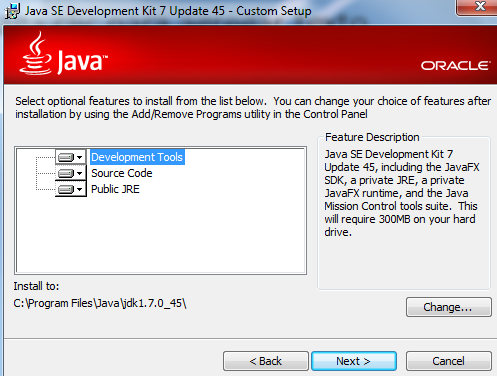
\includegraphics[scale=.4]{images/instalaciones/java/img_java_4}
		\caption{Selección de herramientas de instalación.}
	\end{center}
\end{figure}

Al dar clic en siguiente nos muestra una pantalla del progreso de
descarga según a instalar Productos de Java que es la primer ventana del menú,
lo cual desplegará la siguiente ventana.

\begin{figure}[H]
	\begin{center}
		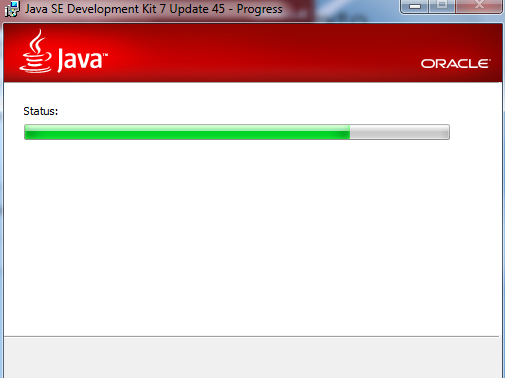
\includegraphics[scale=.4]{images/instalaciones/java/img_java_5}
		\caption{Estatus de descarga del aplicativo.}
	\end{center}
\end{figure}

Posteriormente
comenzará a instalarse la máquina virtual de java que habíamos descargado en los
pasos anteriores, este procedimiento puede tardar dependiendo de los recursos de
nuestro equipo de cómputo.

\begin{figure}[H]
	\begin{center}
		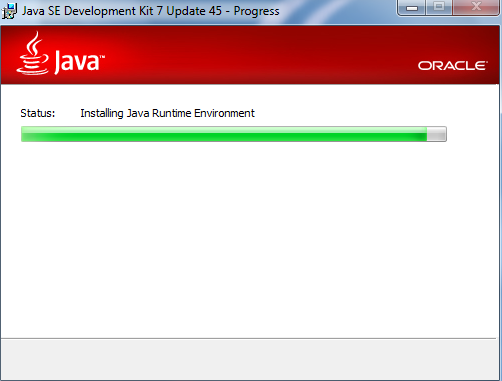
\includegraphics[scale=.4]{images/instalaciones/java/img_java_6}
		\caption{Proceso de instalación de Java runtime Edition.}
	\end{center}
\end{figure} 

En el siguiente paso nos preguntará
si deseamos instalar el JRE de la máquina virtual, obviamente decimos que sí.

\begin{figure}[H]
	\begin{center}
		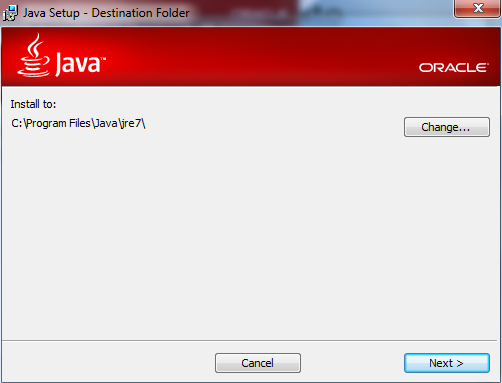
\includegraphics[scale=.4]{images/instalaciones/java/img_java_7}
		\caption{Selección de la carpeta de instalación.}
	\end{center}
\end{figure} 

Comenzará a instalar los componentes del JDK, esto puede tardar
varios minutos así que no desesperen y vayan a preparase una taza de café.

\begin{figure}[H]
	\begin{center}
		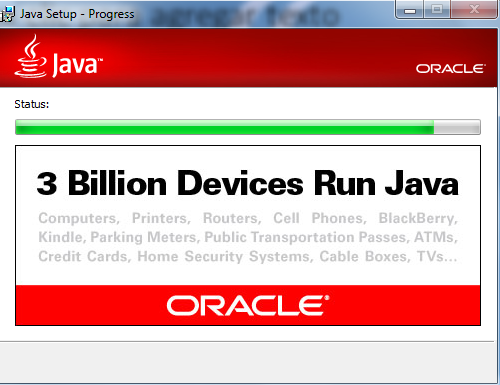
\includegraphics[scale=.4]{images/instalaciones/java/img_java_8}
		\caption{Proceso de instalación.}
	\end{center}
\end{figure}

Hasta este momento tenemos instalado nuestro JDK, pero esto no es
suficiente si queremos que nuestro equipo de cómputo pueda realizar sistemas
informáticos, por esa razón tenemos que decirle a nuestro pc que pueda generar
archivos .class de la siguiente manera. Primero damos clic derecho en equipo y
elegimos propiedades, como en la siguiente imagen:

\begin{figure}[H]
	\begin{center}
		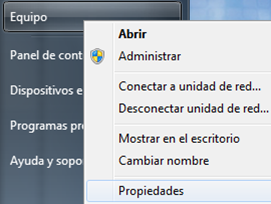
\includegraphics[scale=.4]{images/instalaciones/java/img_java_9}
		\caption{Menú de propiedades de Windows.}
	\end{center}
\end{figure}

Nos mostrara
un cuadro de dialogo en el cual del lado izquierdo contiene un menú donde
nosotros seleccionaremos Configuración Avanzada del Sistema.

\begin{figure}[H]
	\begin{center}
		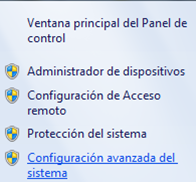
\includegraphics[scale=.4]{images/instalaciones/java/img_java_10}
		\caption{Selección de la configuración del sistema de Windows.}
	\end{center}
\end{figure}

Nuevamente nos abrirá un cuadro de dialogo donde seleccionamos la pestaña
Opciones Avanzadas y elegimos el botón variables de entorno.

\begin{figure}[H]
	\begin{center}
		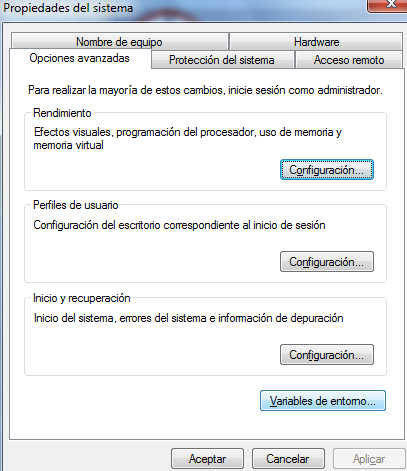
\includegraphics[scale=.4]{images/instalaciones/java/img_java_11}
		\caption{Ventana para seleccionar la configuración de variables de entorno.}
	\end{center}
\end{figure}

En el siguiente cuadro de diálogo tenemos que tener mucho cuidado ya que cada
vez que iniciamos nuestro pc estas variables de entorno son las que se encargan
de cargar nuestro sistema operativo así es que si llegáramos a borrar una
variable de esta sección podría no cargar la próxima vez nuestro sistema
operativo. Primero debemos de ubicar la variable Path, la seleccionamos y damos
clic en el botón Editar.

\begin{figure}[H]
	\begin{center}
		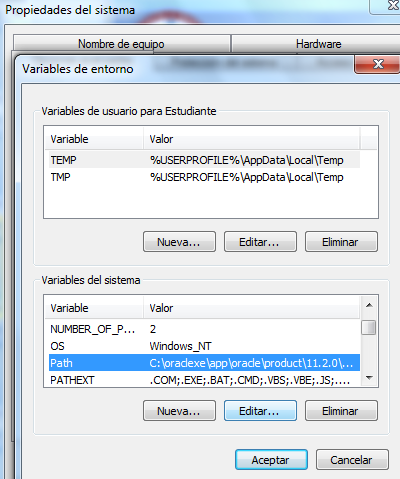
\includegraphics[scale=.4]{images/instalaciones/java/img_java_12}
		\caption{Configuración de la variable $Path$ de Windows.}
	\end{center}
\end{figure}

Debemos de copiar la ruta donde se
instaló nuestro JDK para poder agregarla a las variables de entorno así que
vamos a copiar la ruta.

\begin{figure}[H]
	\begin{center}
		
\includegraphics[scale=.4]{images/instalaciones/java/img_java_13}
		\caption{Carpeta de instalación de java/bin.}
	\end{center}
\end{figure}

En las variables de entorno vamos a
agregar un punto y coma ";" pegamos la ruta que copiamos en el paso anterior y
agregamos nuevamente punto y coma ";" como nota importante no debemos de borrar
ninguna variable de entorno por lo explicado anteriormente.    

\begin{figure}[H]
	\begin{center}
		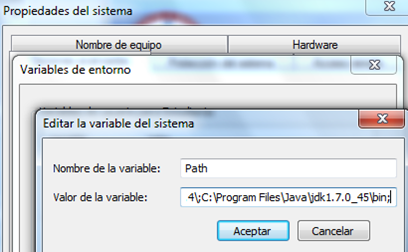
\includegraphics[scale=.4]{images/instalaciones/java/img_java_14}
		\caption{Actualización de la variable $Path$ de Windows con la dirección de 
		la carpeta de instalación de Java.}
	\end{center}
\end{figure}

Aceptamos todas las ventanas que abrimos anteriormente.\\ 
Una vez realizado los
pasos descritos anteriormente es hora de verificar que los hayamos realizado
correctamente. Abrimos una ventana de consola para ello vamos a inicio <<
accesorios >> símbolo de sistema y escribimos el comando java y damos enter.
Nos debe de mostrar muchas líneas describiendo el comando java como se muestra a
continuación. Si nos arrojara un error repetir los pasos anteriores hasta lograr
el objetivo.    

\begin{figure}[H]
	\begin{center}
		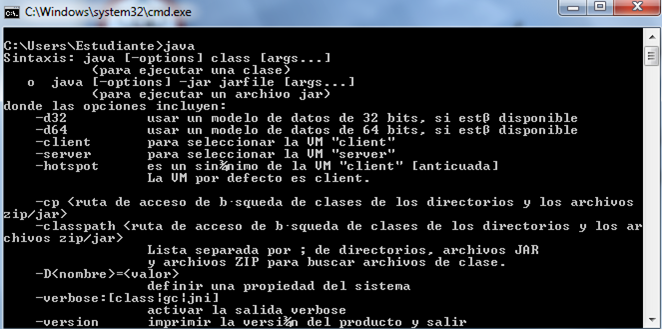
\includegraphics[scale=.4]{images/instalaciones/java/img_java_15}
		\caption{Verificación del comando \textit{java} en la terminal.}
	\end{center}
\end{figure}
 
Ahora escribiremos el comando javac y de la misma
manera que el comando anterior nos debe de describir este comando.\\     

\begin{figure}[H]
	\begin{center}
		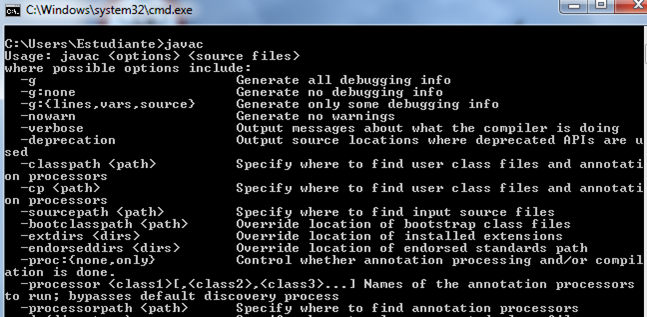
\includegraphics[scale=.4]{images/instalaciones/java/img_java_16}
		\caption{Verificación del comando \textit{javac} en la terminal.}
	\end{center}
\end{figure}

\subsection{Eclipse} 
%% Instalacion de eclipse Empezaremos con la instalación de
Eclipse. Ve a: $http://www.eclipse.org/downloads/ $

\begin{figure}[H]
	\begin{center}
		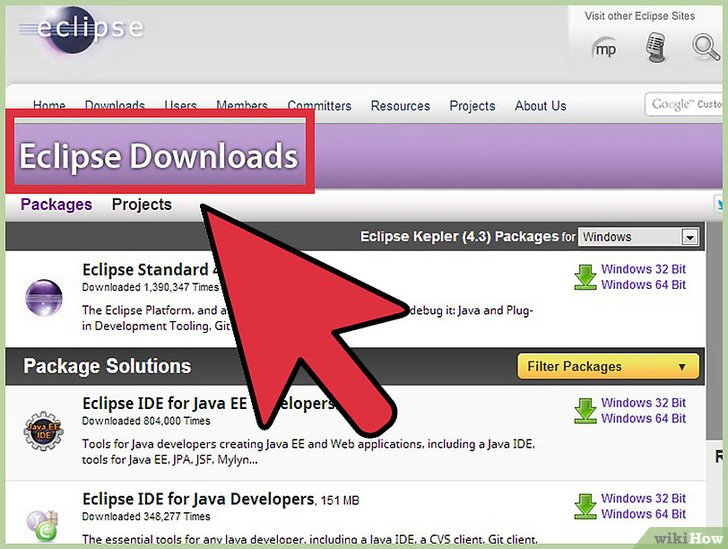
\includegraphics[scale=.4]{images/instalaciones/eclipse/img_eclipse_1}
		\caption{Descarga de eclipse desde la página oficial de eclipse.}
	\end{center}
\end{figure}

 Para los
usuarios de Windows, tendrás que saber qué versión de sistema operativo tienes.
Si tu computadora es de 64-bit, selecciona Windows 64 y si es de 32-bit,
selecciona Windows 32 bit. 

\begin{figure}[H]
	\begin{center}
		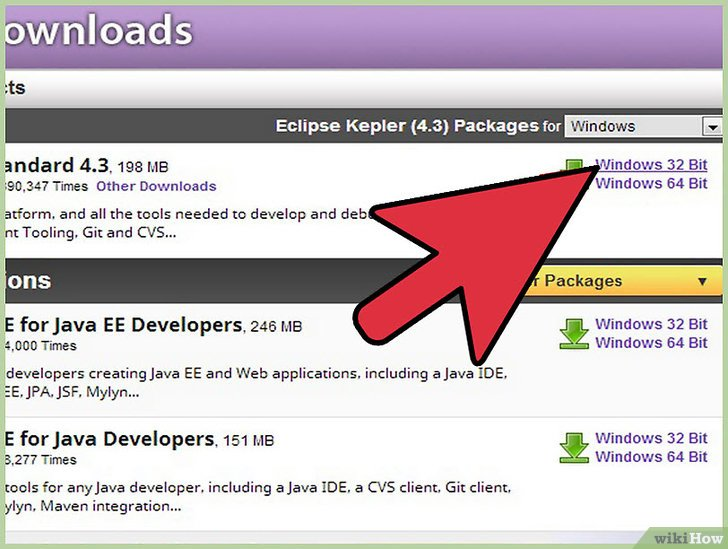
\includegraphics[scale=.4]{images/instalaciones/eclipse/img_eclipse_2}
		\caption{Selección del tipo de sistema operativo dónde se ejecutará la aplicación.}
	\end{center}
\end{figure}

Una vez que descargues el archivo
de Eclipse, necesitarás descomprimir el archivo Zip, el cual creará una carpeta
de Eclipse sin comprimir. Debes extraer el archivo a la raíz de la unidad C:\ ,
así creando la carpeta 
C:\ eclipse , o sólo muévelo o esa carpeta después de
extraerlo. Ya que Eclipse no tiene algún instalador, habrá un archivo dentro de
la carpeta de Eclipse llamado eclipse.exe ( ). Puedes hacer doble clic en el
archivo para ejecutar Eclipse.

\begin{figure}[H]
	\begin{center}
		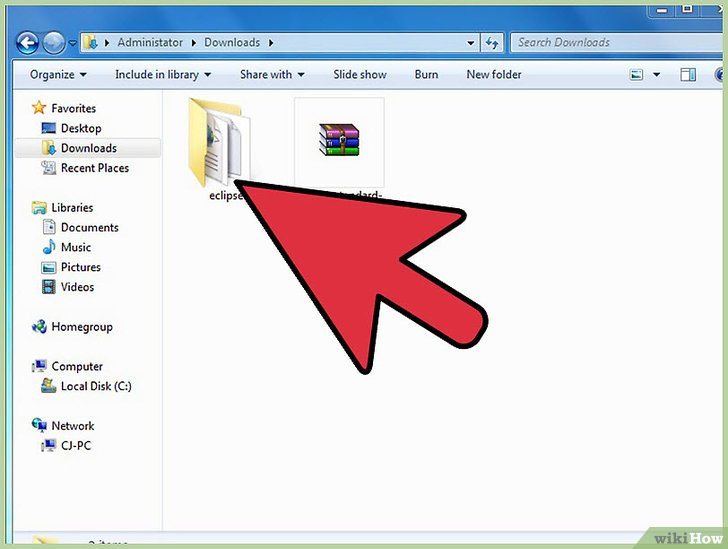
\includegraphics[scale=.4]{images/instalaciones/eclipse/img_eclipse_3}
		\caption{Archivo descomprimido de la descarga.}
	\end{center}
\end{figure} 

\begin{figure}[H]
	\begin{center}
		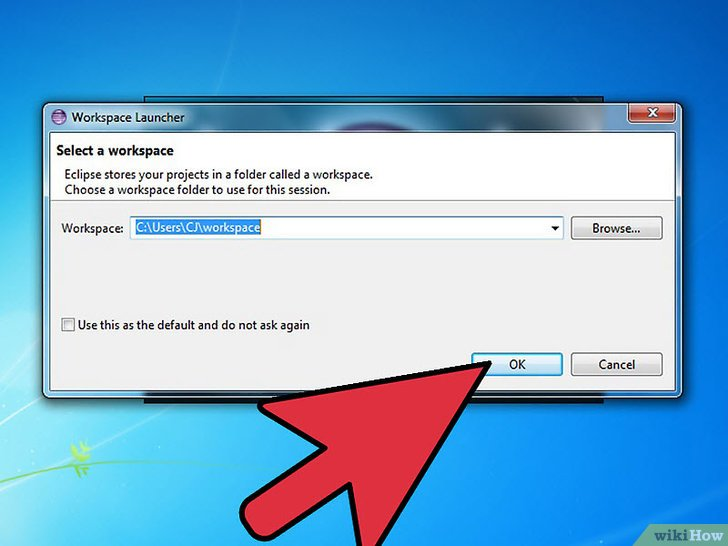
\includegraphics[scale=.4]{images/instalaciones/eclipse/img_eclipse_4}
		\caption{Inicio de un nuevo entorno de trabajo.}
	\end{center}
\end{figure} 
